\section{Understanding Intermediate Representations}
\label{sec:intermediate-computation}

This section explores interpreting hidden activations directly in natural language. In contrast to feature extraction and circuit discovery (Sections~\ref{sec:sae} and \ref{sec:circuit}), which extract features or their interactions from model representations (activations), the methods we will discuss in this section treat the activation itself as the object of interpretation. They use language models or other natural-language-based methods to describe or elicit the encoded information, without intervening on or decomposing the underlying activation. This paradigm provides a direct interface between model activations and natural-language explanations, making it particularly accessible and understandable for human users.


\subsection{Logit Lens: Tracing Predictions Through Depth}
\label{sec:logit-lens}

\begin{definitionbox}[Logit Lens (Figure~\ref{fig:logitlens})]
Logit lens~\citeem{nostalgebraist2020interpretinggpt} applies the model's unembedding matrix to activations at intermediate layers, revealing what the model \emph{would predict} if computation stopped at that layer. For a hidden activation $h_\ell$ at layer $\ell$, logit lens computes:
\[
\text{logits}_\ell = W_U h_\ell,
\]
where $W_U$ represents the model's unembedding matrix. Applying it across layers reveals the prediction trajectory, showing when and where the model commits to specific outputs~\citeem{nostalgebraist2020interpretinggpt}.
\end{definitionbox}

Logit lens (Figure~\ref{fig:logitlens}) provides intuitive insight into the model's decision-making process across depth. Experimental results show that early layers tend to produce diffuse predictions, while later layers progressively narrow them towards the final output, though exceptions exist. For example, in a twelve-layer language model processing the sequence \texttt{A B C A B}, the logit lens may reveal that the token \texttt{C} enters the top-20 candidates at layer 6 and is progressively amplified, eventually becoming the top-ranked token at the final layer. Conversely, for induction tasks in complex linguistic patterns, early and middle layers may show a flat probability distribution across many tokens, with the model converging to a specific prediction only in the last few layers.

\begin{figure}[tb]
\centering
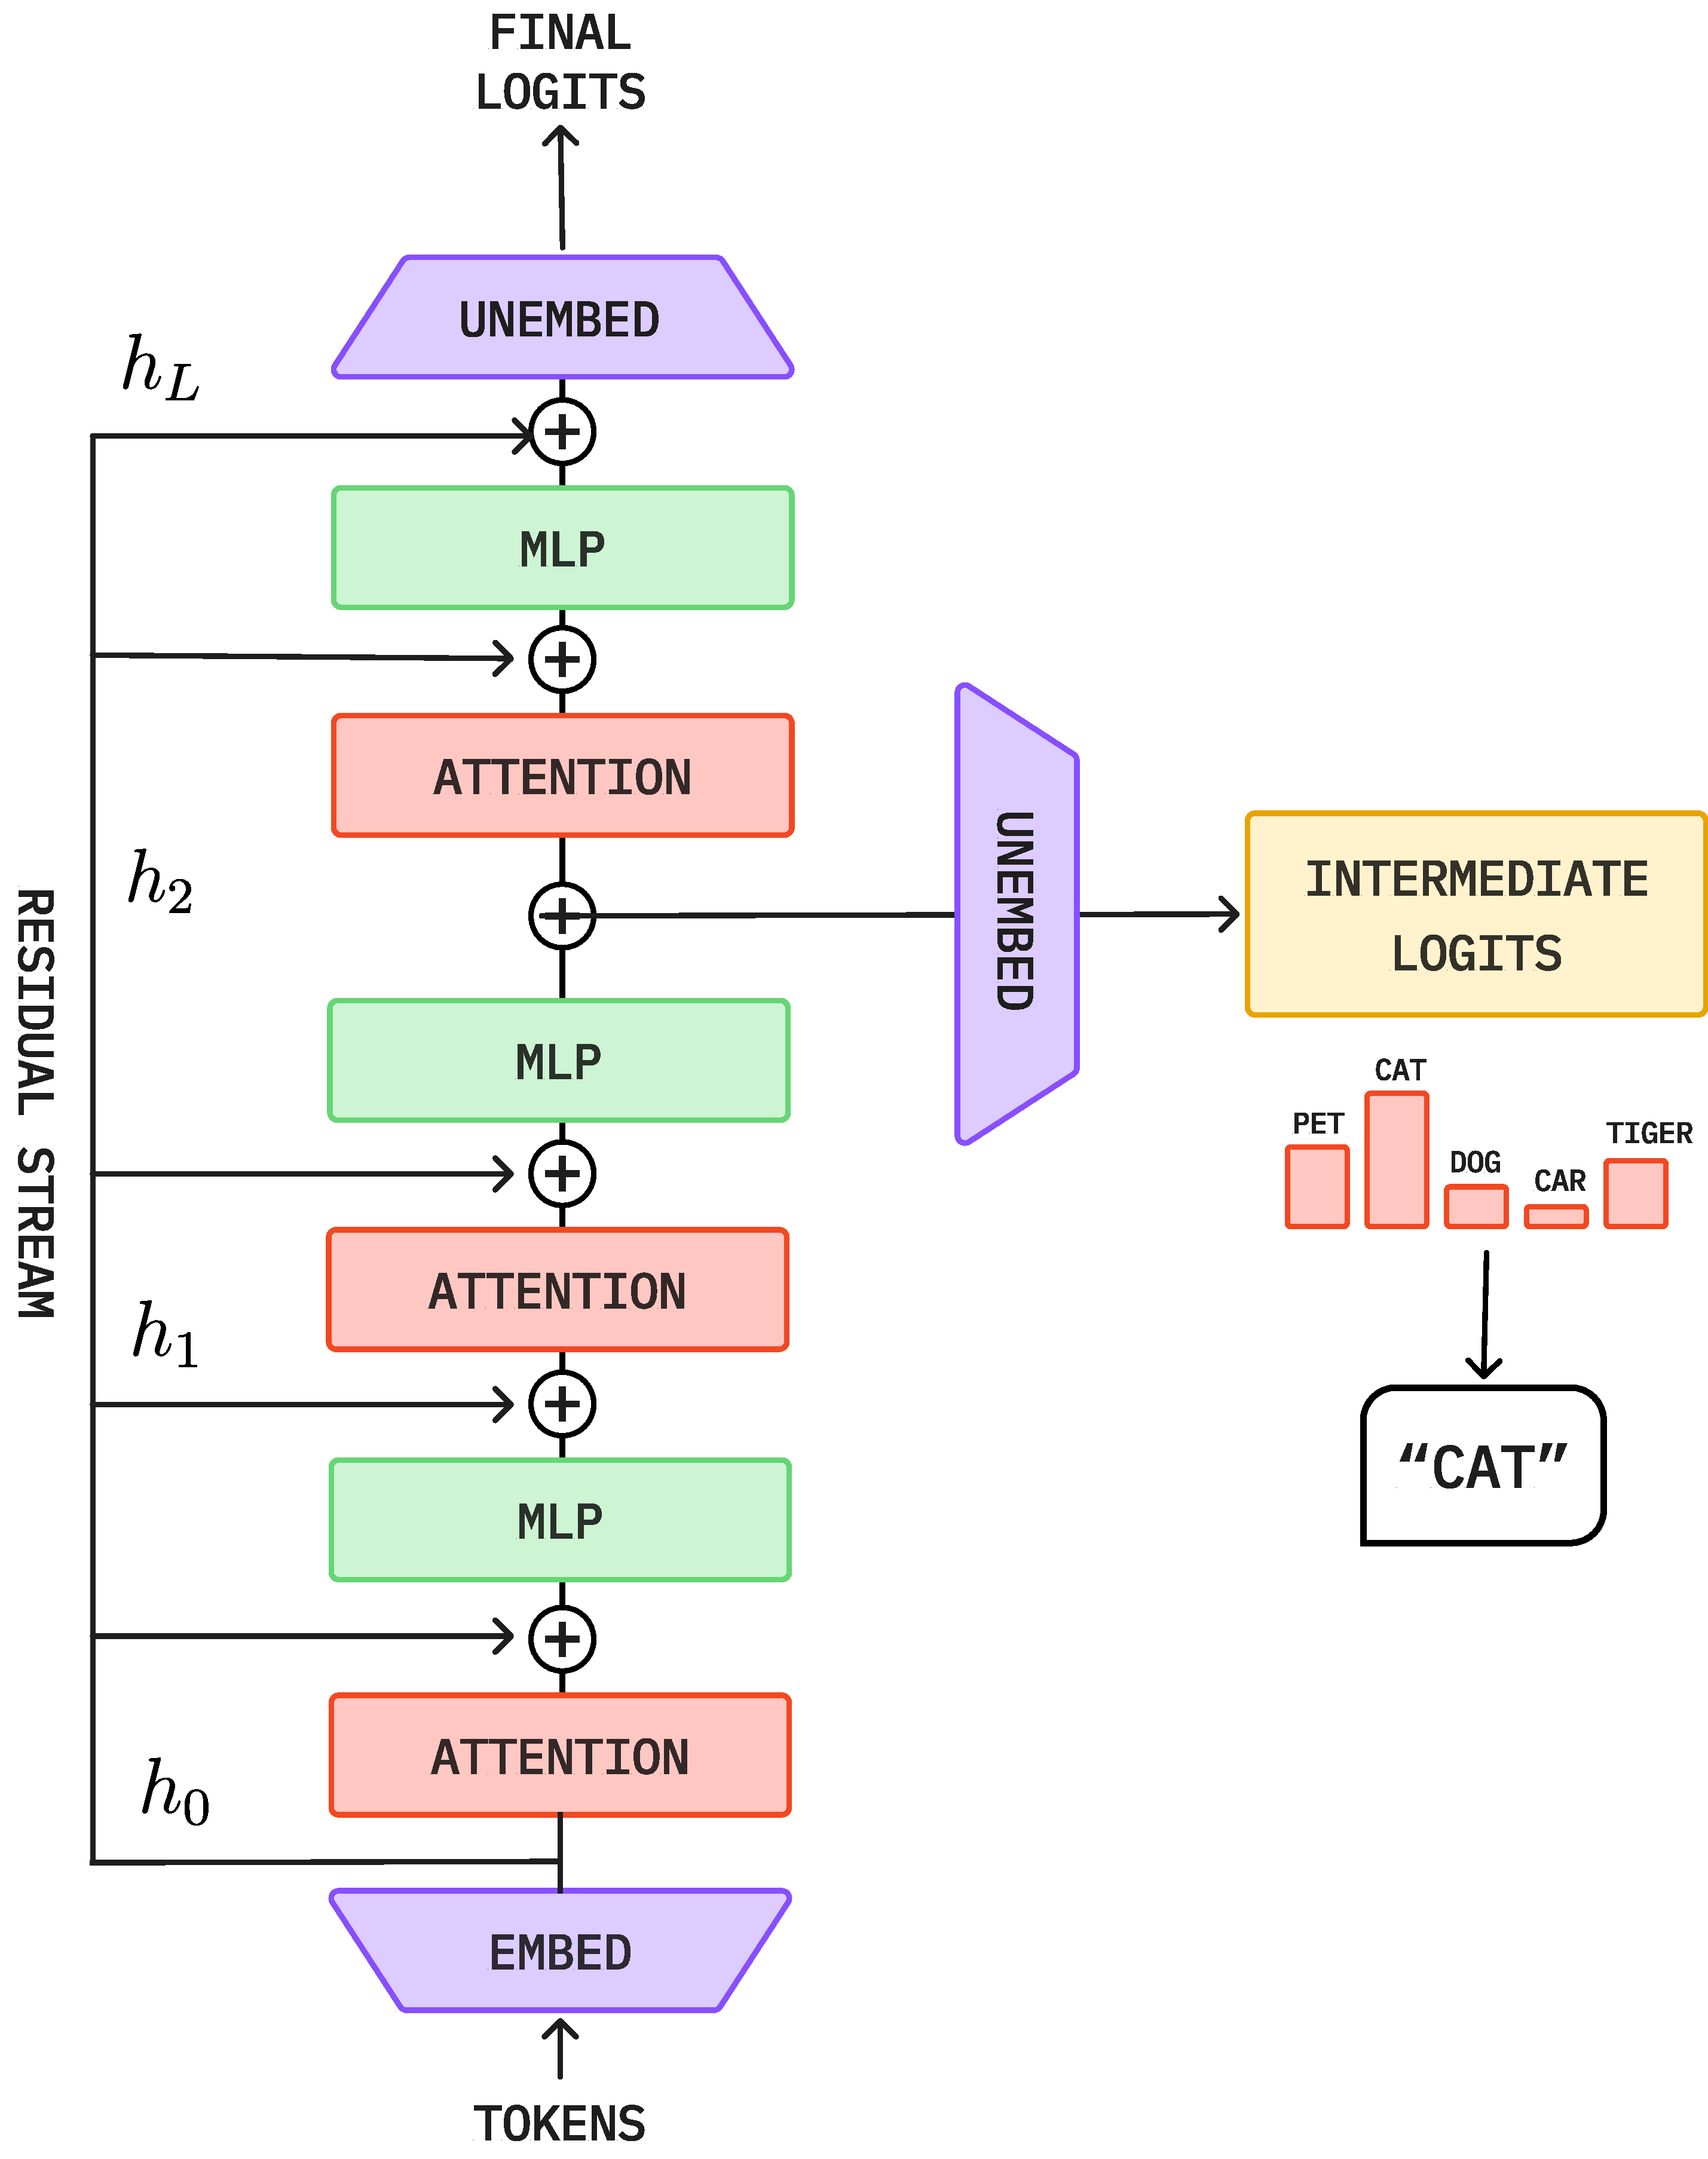
\includegraphics[width=0.5\linewidth]{figs/8_Logit_Lens.pdf}
\caption{\textbf{Logit Lens.} Logit lens provides a window into a model's intermediate state by applying the final unembedding layer directly to the residual stream at earlier layers ($h_1, h_2, \ldots$). This allows users to see which tokens the model is ``considering'' mid-computation, such as the emergence of the concept ``CAT'' before the final output layer is reached.}
\label{fig:logitlens}
\end{figure}

\paragraph{Limitations of Vanilla Logit Lens.}
The vanilla logit lens has a critical limitation: applying the unembedding matrix to intermediate activations assumes that the hidden state is in a format that the output layer expects. However, intermediate representations may be organised very differently from output-layer activations. Applying the unembedding matrix to layer-6 activations may extract relevant information but cannot precisely reflect the model's underlying computation at that layer~\citeem{nostalgebraist2020interpretinggpt}.
Furthermore, logit lens is fundamentally correlational rather than causal. It projects the activation into the output vocabulary space without testing the roles decoded tokens play in model computation. In particular, because of the representational mismatch discussed above, decoded tokens represent at most information recoverable from the activation, rather than information used in model computation.

\subsection{Tuned Lens: Learning Per-Layer Transforms}
\label{subsec:tuned-lens}

\begin{definitionbox}[Tuned Lens]
Tuned lens~\citeem{belrose2025elicitinglatentpredictionstransformers} addresses logit lens' concern of representational mismatch by learning per-layer affine transformations that map intermediate activations to the output layer's activation space:
\[
\text{logits}_\ell^{\text{TL}} = W_U (W_\ell h_\ell + b_\ell),
\]
where $W_\ell$ and $b_\ell$ are learned affine transformations for layer $\ell$. These transforms are trained to minimise the divergence between the tuned lens' predicted distribution $p_\ell^{\text{TL}} = \operatorname{softmax}(\text{logits}_\ell^{\text{TL}})$ and the model output distribution $p_{\text{final}}$ via:
\[
\min_{W_\ell,b_\ell}\mathbb{E}_{x\sim\mathcal{D}}\big[\,\mathrm{KL}(p_{\text{final}}(x)\;\|\;p_\ell^{\text{TL}}(x))\big].
\]
\end{definitionbox}
As a result, the unembedding matrix can extract relevant information from each layer's activations more effectively.

\paragraph{Limitations of Tuned Lens.}
Although tuned lens mitigates representational mismatch, it still inherits several fundamental limitations. First, the decoding paradigm remains inherently correlational rather than causal; decodable information does not imply a causal role in the model's prediction. Second, similar to logit lens, tuned lens is primarily designed to answer \emph{what the model is likely to predict} rather than \emph{what the model is internally computing}. The learned layer-specific transformations that align intermediate representations with the final prediction space may obscure intermediate computational steps and produce predictions that resemble the model's final output. Empirical evidence also shows that it skips intermediate computation more aggressively than logit lens~\citeem{jlens}.

\subsection{Jacobian Lens: Decoding Computational Dispositions}
\begin{definitionbox}[Jacobian Lens]
Jacobian lens (J-lens; \citeemalp{jlens}) adopts a decoding paradigm distinct from logit lens and tuned lens. It uses the Jacobian to characterise how an intermediate representation influences certain model outputs.\\

Let $h_\ell^t$ denote the residual stream at layer $\ell$ and position $t$. A perturbation to $h_\ell^t$ propagates to the final-layer residual stream at every position $t' \geq t$; to first order, this influence is captured by the Jacobian
\[
\frac{\partial h_{\mathrm{final}}^{t'}}{\partial h_\ell^t}.
\]
The lens matrix is defined as the expectation of this Jacobian over prompts and positions:
\[
J_\ell
=
\mathbb{E}_{\,\mathrm{prompt},\,t,\,t' \ge t}
\left[
\frac{\partial h_{\mathrm{final}}^{t'}}
{\partial h_\ell^t}
\right].
\]
J-lens then decodes intermediate representations by
\[
p_\ell^{\mathrm{JL}}
=
\operatorname{softmax}
\!\big(
W_U \operatorname{norm}(J_\ell h_\ell)
\big).
\]

\citetem{jlens} further defined layer-specific concept (token) representations using the rows of $W_U J_\ell$, called \emph{J-lens vectors}. The inner product between a J-lens vector and $h_\ell$ measures how strongly the current activation will promote the corresponding token in model outputs.
\end{definitionbox}

Unlike logit lens and tuned lens, which primarily estimate which token the model is likely to predict next, J-lens characterises how current representations influence model outputs. It aims to answer \emph{what the model is internally computing} rather than merely \emph{what the model is going to predict}. J-lens has been found useful for analysing tasks that require multi-step reasoning, latent planning, or other forms of extended computation~\citeem{jlens}.

Furthermore, the defined J-lens vectors are a useful medium for intervention. They can serve as steering vectors to shift model behaviour towards or away from the corresponding concepts. In contrast, interventional utility is largely absent from logit lens and tuned lens, which are primarily decoding tools.

\paragraph{Limitations of Jacobian Lens.}
J-lens still faces several limitations that warrant further investigation. First, like logit lens and tuned lens, it operates primarily at the token level. However, many semantically meaningful concepts are represented by multiple tokens. For example, the word ``photoperiodism'' may be split into several subword tokens. If only one token (e.g., ``photo'') is visible in J-lens, we cannot tell whether it corresponds to the concept of photoperiodism or to other words. Second, J-lens is found to work best within a certain range of layers, called \emph{J-space}~\citeem{jlens}. Specifically, decoded concepts are most informative in intermediate layers (e.g., approximately 38--92\% of the depth in Claude Sonnet 4.5). In early layers, decoded concepts are noisy and hard to interpret. In later layers, they collapse towards the model's output and are also uninformative. Some recent studies have attempted to address these limitations~\citeem{jlens, blank2026rlens}.










\subsection{Patchscopes: Leveraging the Language Model Itself to Explain Intermediate Representations}
\label{subsec:patchscopes}

\begin{figure}[tb]
\centering
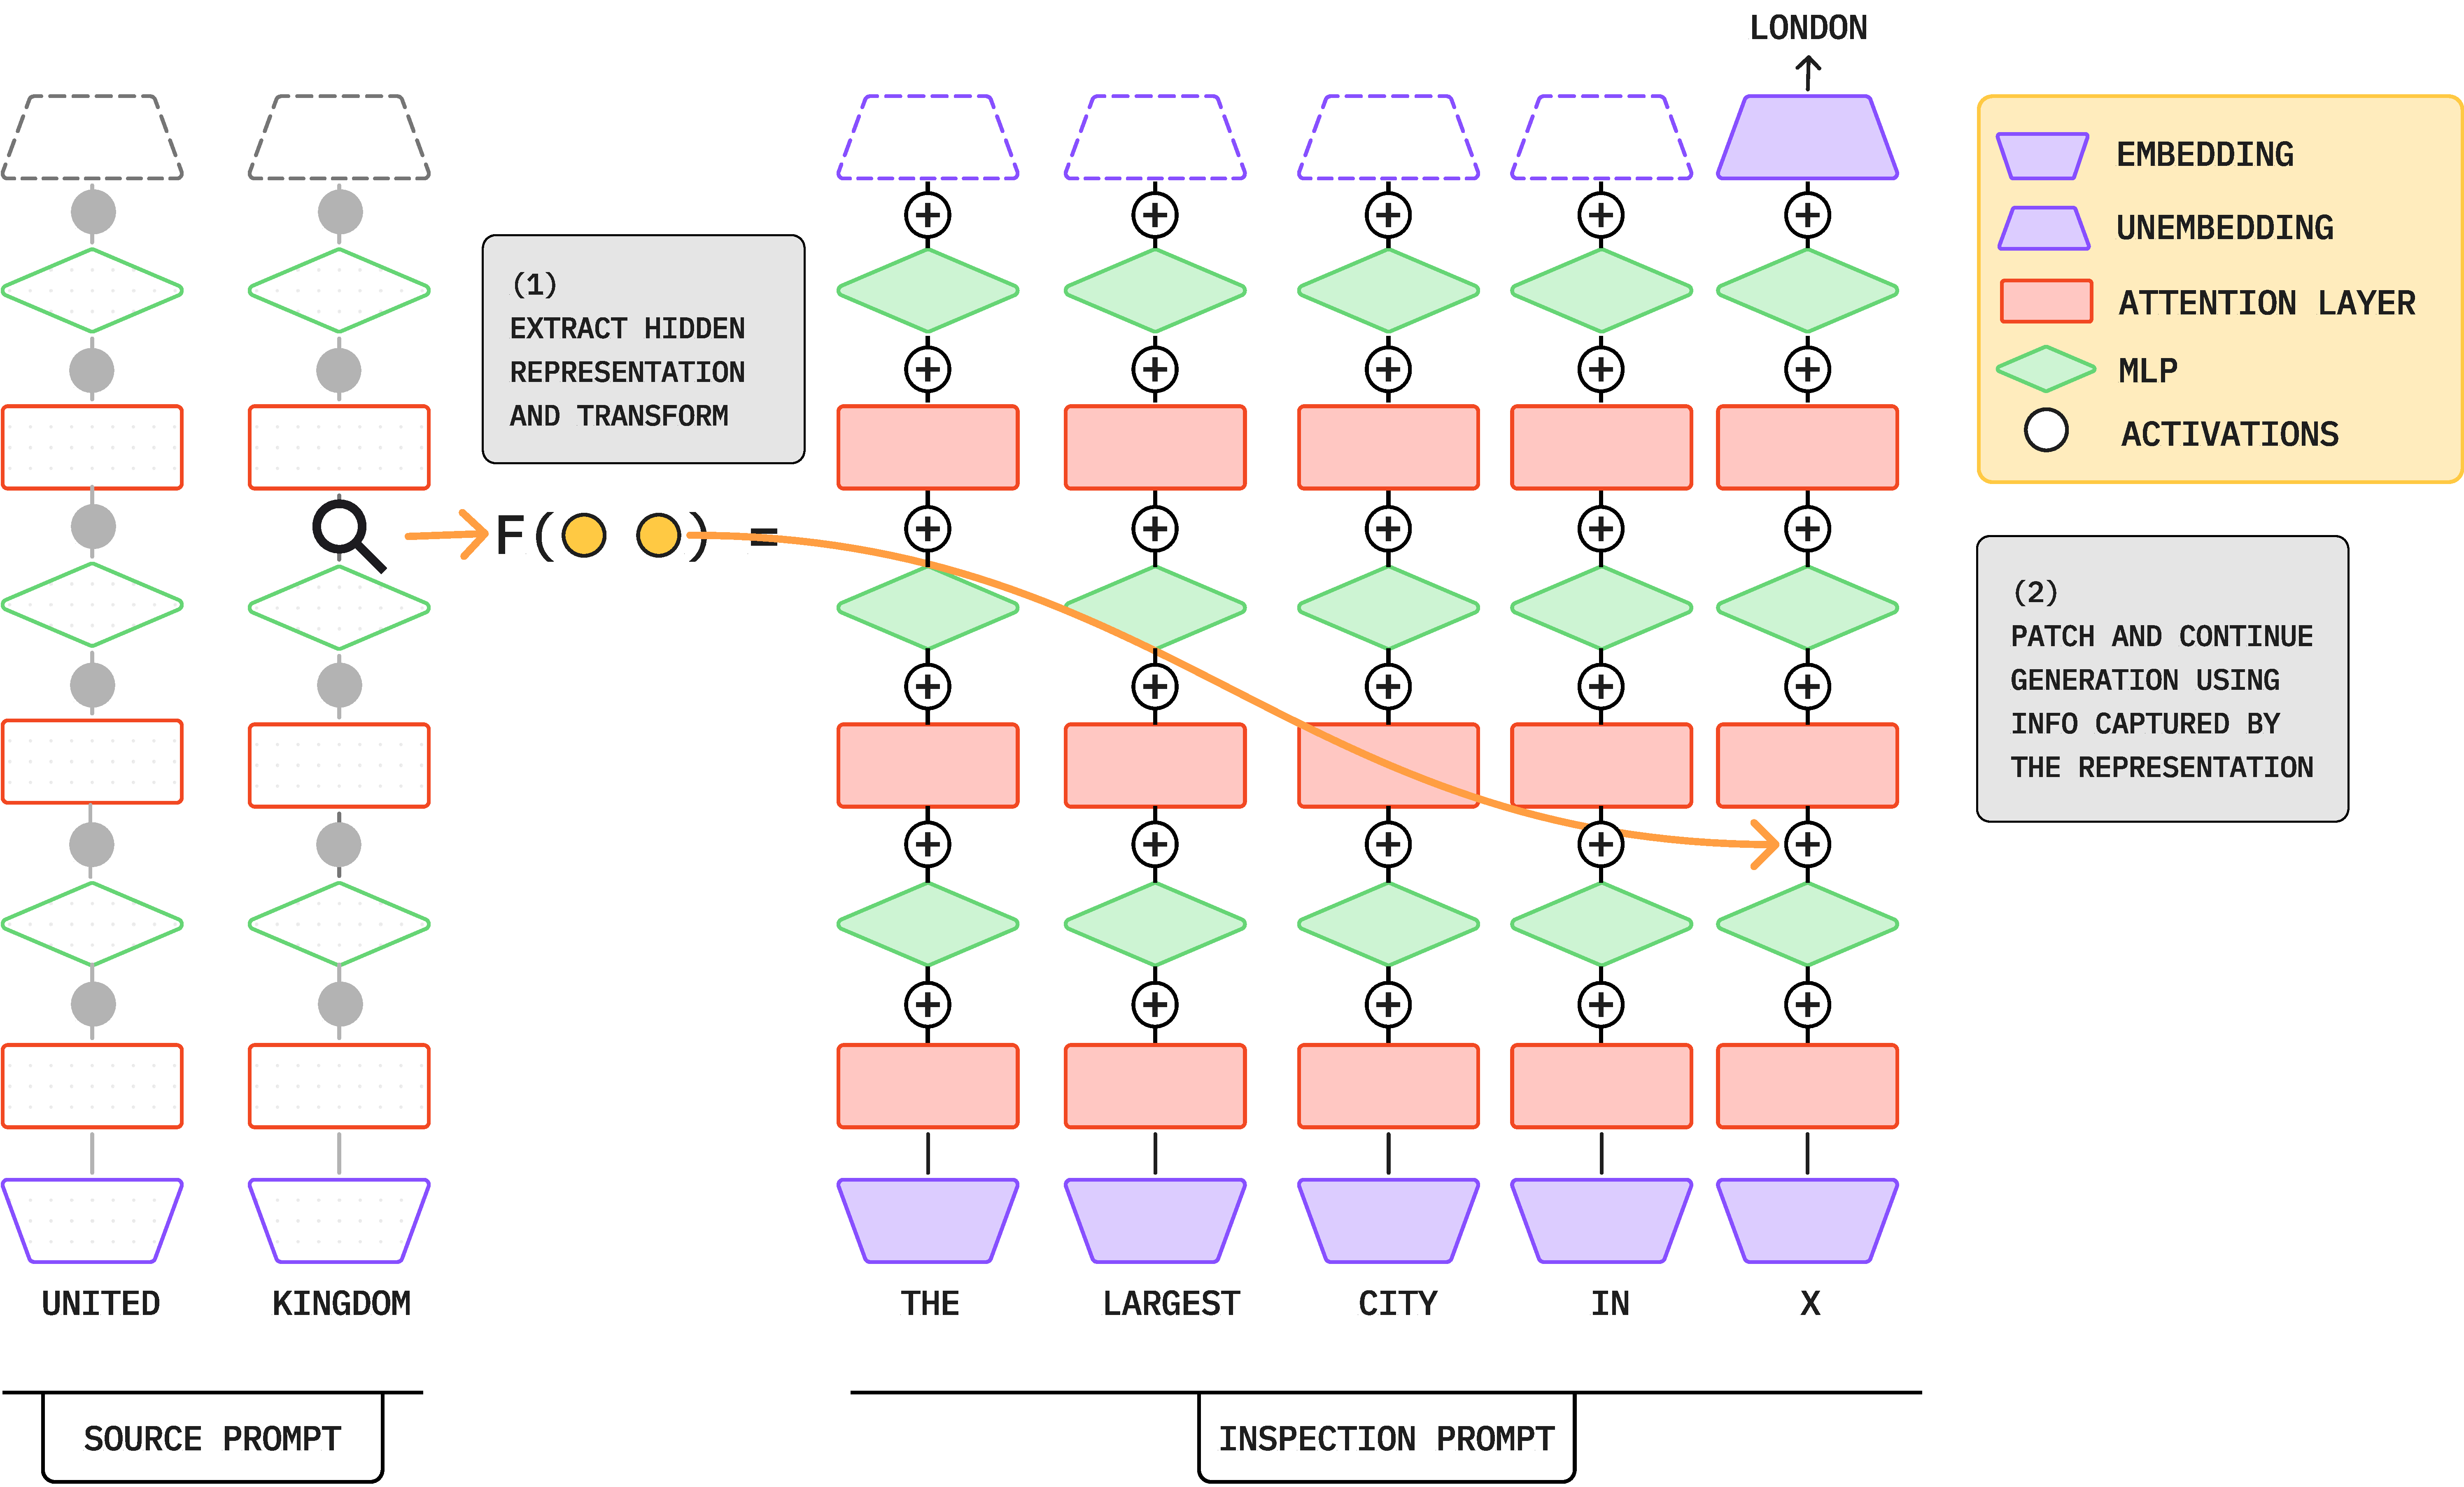
\includegraphics[width=\linewidth]{figs/8_Patchscopes.pdf}
\caption{\textbf{Patchscopes.} Patchscopes extracts the model representation of interest from a source prompt and ``patches'' it into an inspection prompt. By observing changes in model output, users can examine what information the representation contains. For example, in this figure we can observe whether the representation of ``United Kingdom'' correctly triggers ``London'' as the largest city.}
\label{fig:patchscopes}
\end{figure}

\begin{definitionbox}[Patchscopes (Figure~\ref{fig:patchscopes})]
Patchscopes~\citeest{patchscopes} leverages the expressive capacity of language models to translate their internal representations into natural-language explanations. Let $h^t_\ell$ denote a hidden representation at layer $\ell$ and token position $t$. Patchscopes produces a textual explanation of $h^t_\ell$, denoted as $e(h^t_\ell)$, by
\[
e(h^t_\ell) = f_\theta(p_{[h^{t^*}_{\ell^*} \leftarrow h^t_\ell]}),
\]
where $\ell^*$ and $t^*$ specify the layer and token position to which the representation is patched, and $p$ is an \emph{elicitation prompt} designed to encourage the language model $f_\theta(\cdot)$ to decode the patched representation into text expressing the contained information.\\

For example, consider the prompt illustrated in Figure 1 of \citetest{patchscopes}:
\[
p = \text{``cat$\rightarrow$cat; 135$\rightarrow$135; hello$\rightarrow$hello; ?''},
\]
where $t^*$ corresponds to the position of the token ``?''. The notation $[h^{t^*}_{\ell^*} \leftarrow h^t_\ell]$ indicates that, during the forward pass of $f_\theta(\cdot)$ on $p$, the hidden representation at layer $\ell^*$ and position $t^*$ is replaced with $h^t_\ell$. As a result, the model can reveal information encoded in $h^t_\ell$ through its prediction for the next token at the ``?'' position.
\end{definitionbox}

Because the mapping from intermediate representations to natural language may be too complex to be captured by an affine transformation, Patchscopes (Figure~\ref{fig:patchscopes}) extends the paradigm of logit lens and tuned lens by \emph{delegating the representation-to-text transformation to the language model itself}\footnote{A concurrent work, SelfIE~\citeest{selfie}, explores a similar direction. While we focus on Patchscopes as a reference framework, both methods share closely related motivations and methodologies.}. In this view, the language model acts as an \emph{activation decoder}. Crucially, Patchscopes relies on the model's learned, generalisable text-generation capabilities to map internal activations to natural language.

\paragraph{Limitations of Patchscopes.}
A key limitation of Patchscopes is that injecting an external representation into an elicitation prompt can shift the model's internal activations into an out-of-distribution (OOD) regime. This is expected, as the decoder is a standard pretrained language model not explicitly trained for representation-to-text decoding. Although the model may still surface salient information from the patched representation, the decoding process can degrade, and critical aspects of the original representation may be distorted or lost.

\subsection{LatentQA: Fine-Tuning the Language Model as an Activation Verbaliser}
\label{subsec:latentqa}

\begin{definitionbox}[LatentQA (Figure~\ref{fig:latentqa})]
LatentQA~\citeest{pan2024latentqateachingllmsdecode} frames representation decoding as a supervised learning problem via Latent Interpretation Tuning (LIT), fine-tuning an activation verbaliser to perform representation-to-text verbalisation. The core step of LIT is to construct a fine-tuning dataset $D$ consisting of samples $(h^t_\ell, q, a)$, where $h^t_\ell$ is a cached hidden representation from a target model, and $(q, a)$ is a question--answer pair that queries the information encoded in $h^t_\ell$.\\

Specifically, $h^t_\ell$ denotes the activation at layer $\ell$ and token position $t$ when the target model processes a ``control prompt'' designed to embed a specific attribute or concept into the representation. An example control prompt from Figure 13 of \citetest{pan2024latentqateachingllmsdecode} is:
\[
\text{``In your next reply, please try to evoke a brief sense of triumphant hubris.''}
\]
If $h^t_\ell$ is defined as the activation at layer $\ell$ corresponding to the final token (``.'') of this prompt, the resulting representation is expected to encode the instruction to respond with triumphant hubris. In this case, a corresponding question--answer pair may be:
\[
q = \text{``In what way does the assistant craft its responses to the user?''}
\]
\[
a = \text{``The assistant crafts responses that briefly highlight a sense of self-assured victory.''}
\]
Both the control prompt and the $(q, a)$ pair are generated by prompting an off-the-shelf proprietary language model~\citeest{pan2024latentqateachingllmsdecode}.
\end{definitionbox}

LatentQA (Figure~\ref{fig:latentqa}) addresses the OOD issue inherent in Patchscopes-style methods by explicitly fine-tuning the activation verbaliser on the representation-to-text decoding task. Through LIT, the verbaliser learns to ingest and process raw activation vectors directly. Ideally, after being exposed to a sufficiently diverse collection of question--answer pairs over many different representations, the decoder learns \emph{which aspects of the activation to attend to} and \emph{how to verbalise them} conditioned on the query.

\begin{figure}[tb]
\centering
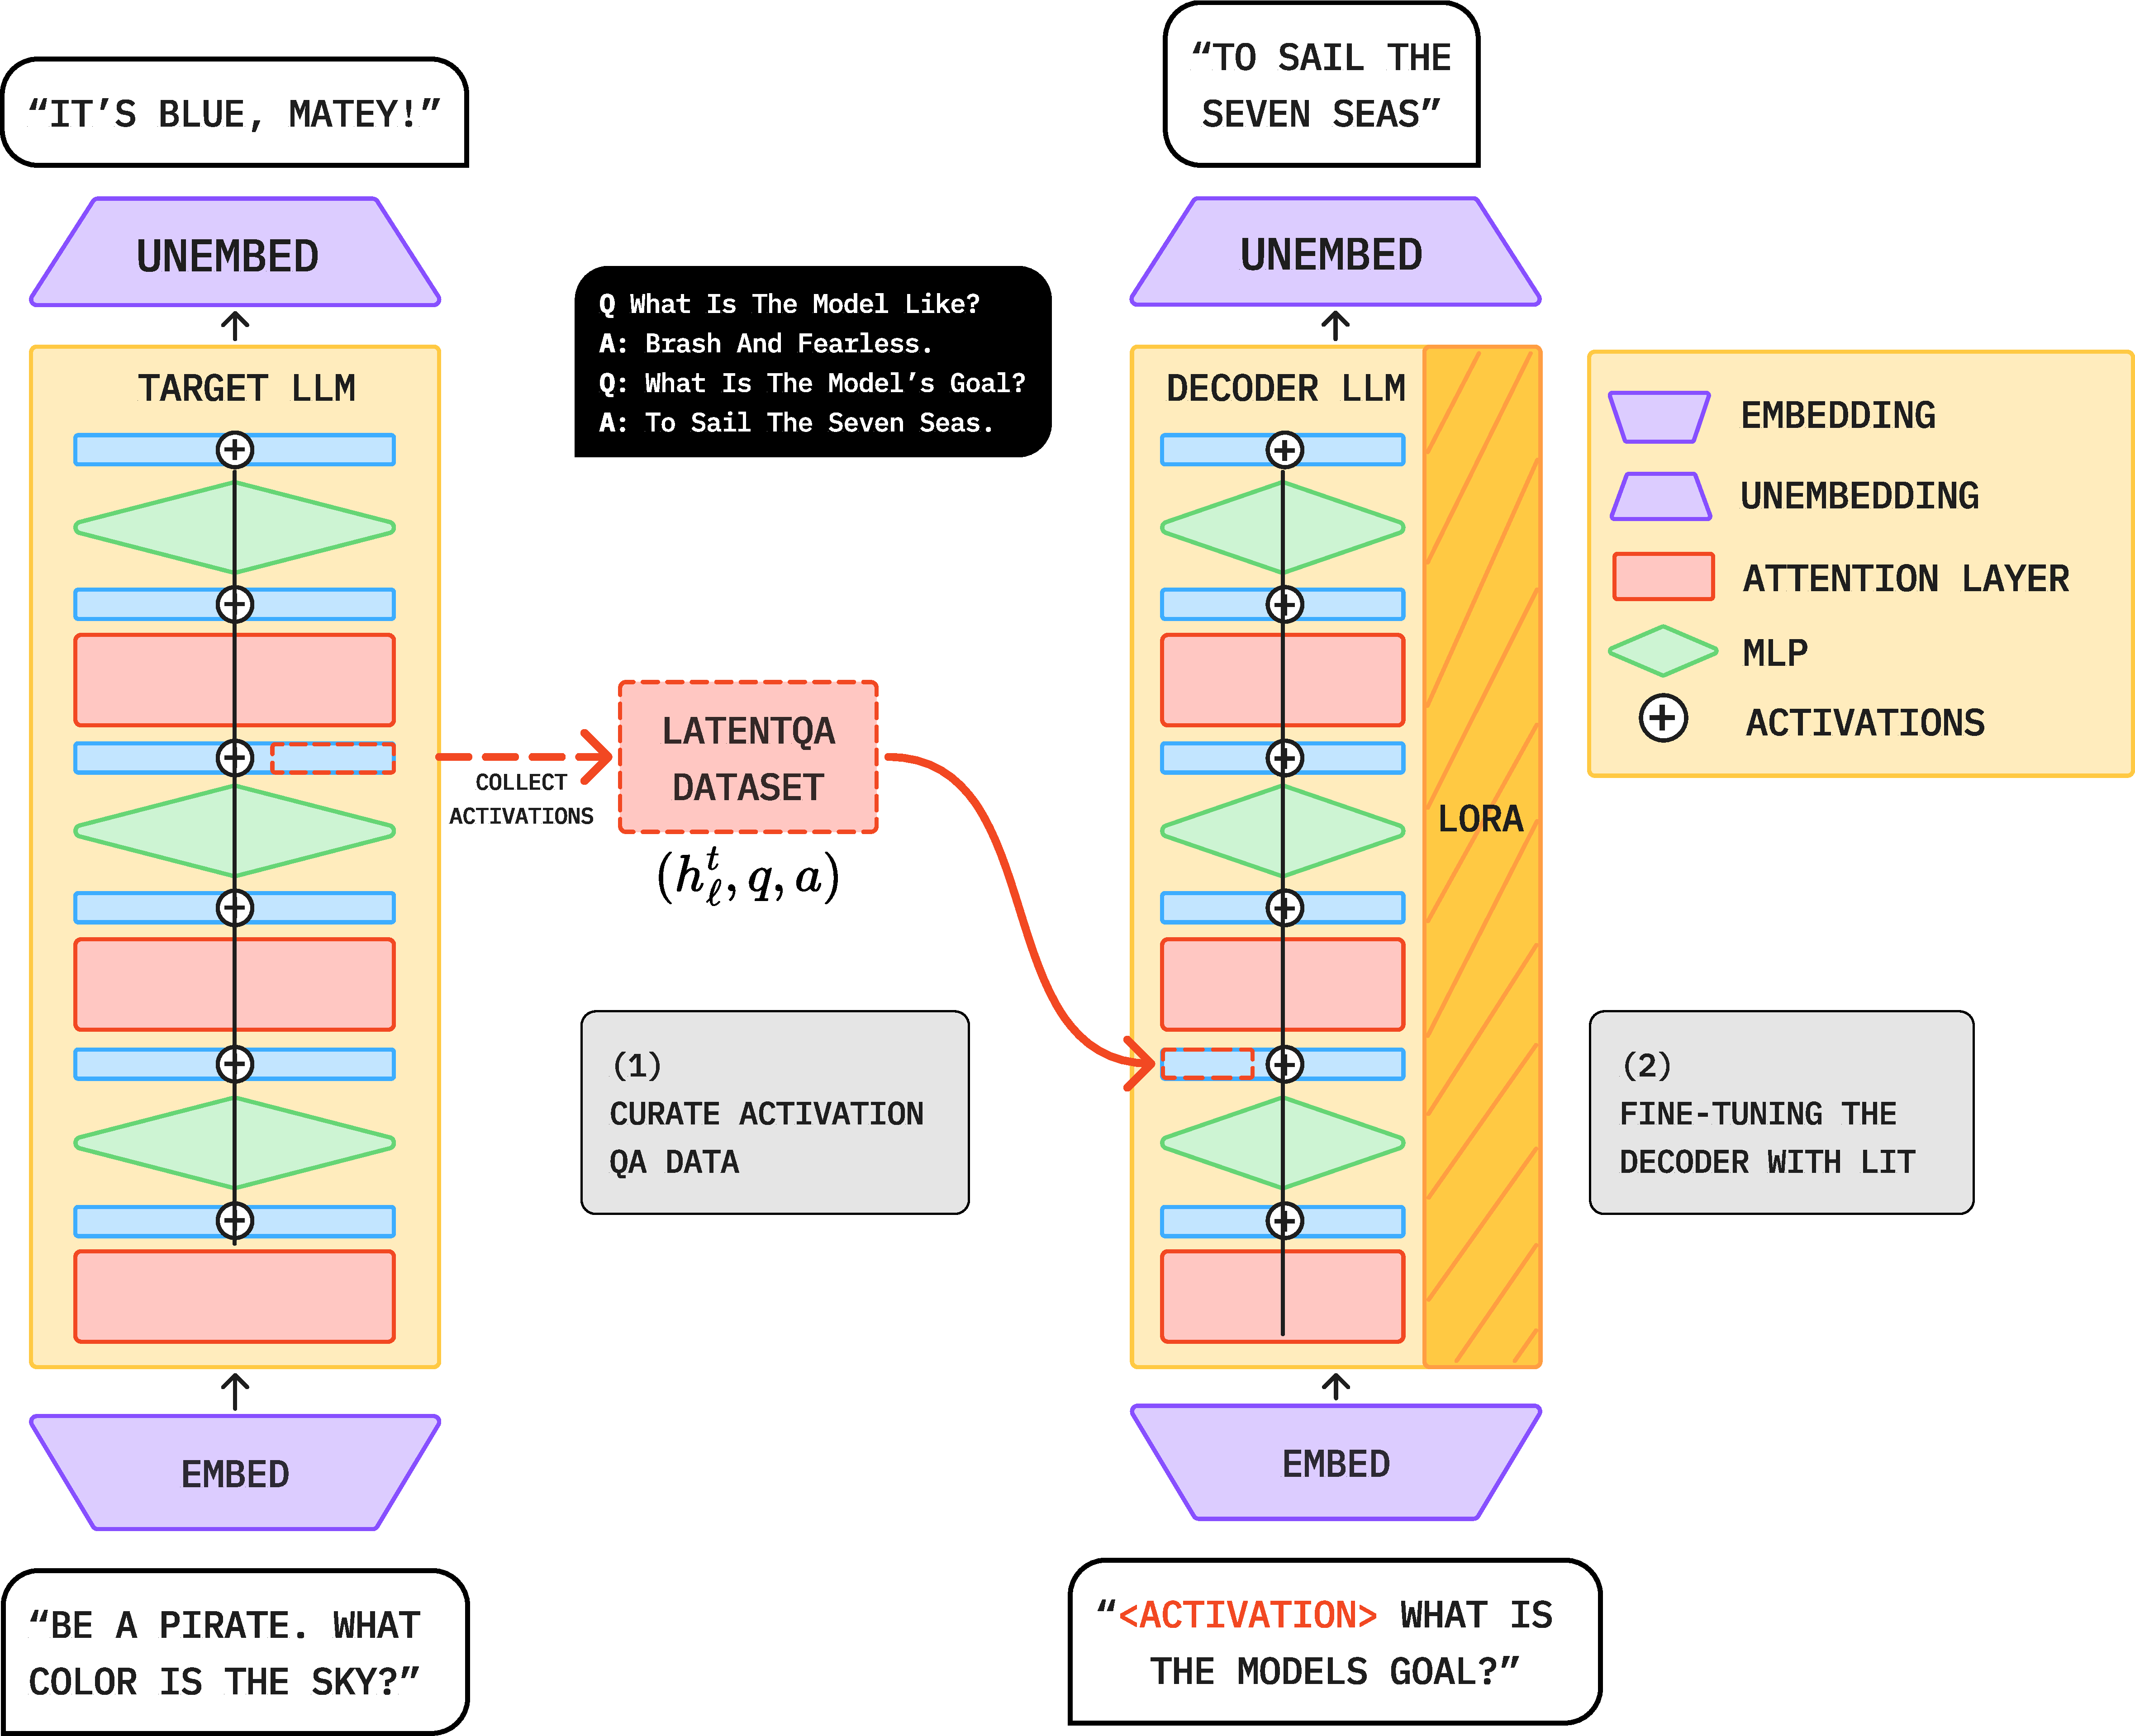
\includegraphics[width=0.8\linewidth]{figs/8_Latent_QA.pdf}
\caption{\textbf{LatentQA.} LatentQA probes the semantic content of hidden representations by training a separate verbaliser model to answer natural-language questions about them. The process involves (1) curating a dataset of activation--question--answer triplets from a target LLM, and (2) fine-tuning a verbaliser to retrieve specific information latent within those activations, such as the model's underlying goals or persona.}
\label{fig:latentqa}
\end{figure}

\paragraph{Limitations of LatentQA.}
LatentQA faces several technical challenges, including the generalisability of the learned representation-to-text mapping. When the fine-tuning dataset $D$ is too small or insufficiently diverse, the verbaliser may memorise superficial correspondences between representations and explanations rather than learning to extract information from representations. Recent approaches, such as Predictive Concept Decoders (PCDs)~\citeem{pcd} and Activation Oracles (AOs)~\citeest{ao}, mitigate this issue by constructing more diverse training datasets.

Another technical challenge is evaluating whether activation-verbalisation models genuinely explain the represented information rather than exploit shortcuts. For example, a verbaliser may implicitly reconstruct the original input to the target model and infer an explanation from it. Recent studies have found that such failure modes are severe and prevalent in existing verbalisers~(\citeestalp{li2026do}; \citeemalp{jakkli2026current}). As a result, strong verbalisation performance alone is insufficient to show that the verbaliser faithfully analysed the internal representations.

\subsection{Probing Classifiers: Capabilities, Critiques, and Causal Limitations}
\label{subsec:probing}

Probing classifiers (Figure~\ref{fig:probing}) are among the most widely used tools for analysing neural network representations. A probe is a classifier trained to predict a property of the input, such as part of speech, sentiment, or entity type, from model activations. High probe accuracy means that the property is decodable from the activations. However, information decodability is a relatively coarse-grained, correlational interpretability claim compared with causal claims about information in model computation. This section reviews probing methodology, its major critiques, and its appropriate role in interpretability research.

As a side note, discovered probe directions can also be used as supervised feature extractors. We discuss this perspective in Section~\ref{subsubsec: supervised_extraction}, including comparisons with SAEs, and in Section~\ref{subsec:steering}, where we discuss their use as steering vectors.

\subsubsection{Standard Probing Methodology}

\begin{definitionbox}[Probing Classifier (Figure~\ref{fig:probing})]
A \emph{probing classifier} is a supervised model trained to predict a target property \(y\) from neural network activations \(h_\ell\) at layer \(\ell\). A \emph{linear probe} follows the form:
\[
\hat{y} = g(W_{\text{probe}} h_\ell + b_{\text{probe}}),
\]
where \(W_{\text{probe}}\) and \(b_{\text{probe}}\) are learned parameters. \(g\), typically an identity function for regression and softmax for classification, maps the probe's raw output to the prediction space. The probe is trained by minimising prediction error on labelled examples \( (h_\ell^{(i)}, y^{(i)}) \). The linear probe tests whether the target property is linearly accessible from the representation. \emph{MLP probes} introduce one or more nonlinear hidden layers instead of $W_{\text{probe}}$ to test whether the property can be retrieved through more expressive nonlinear mappings.
\end{definitionbox}

\begin{figure}[tb]
\centering
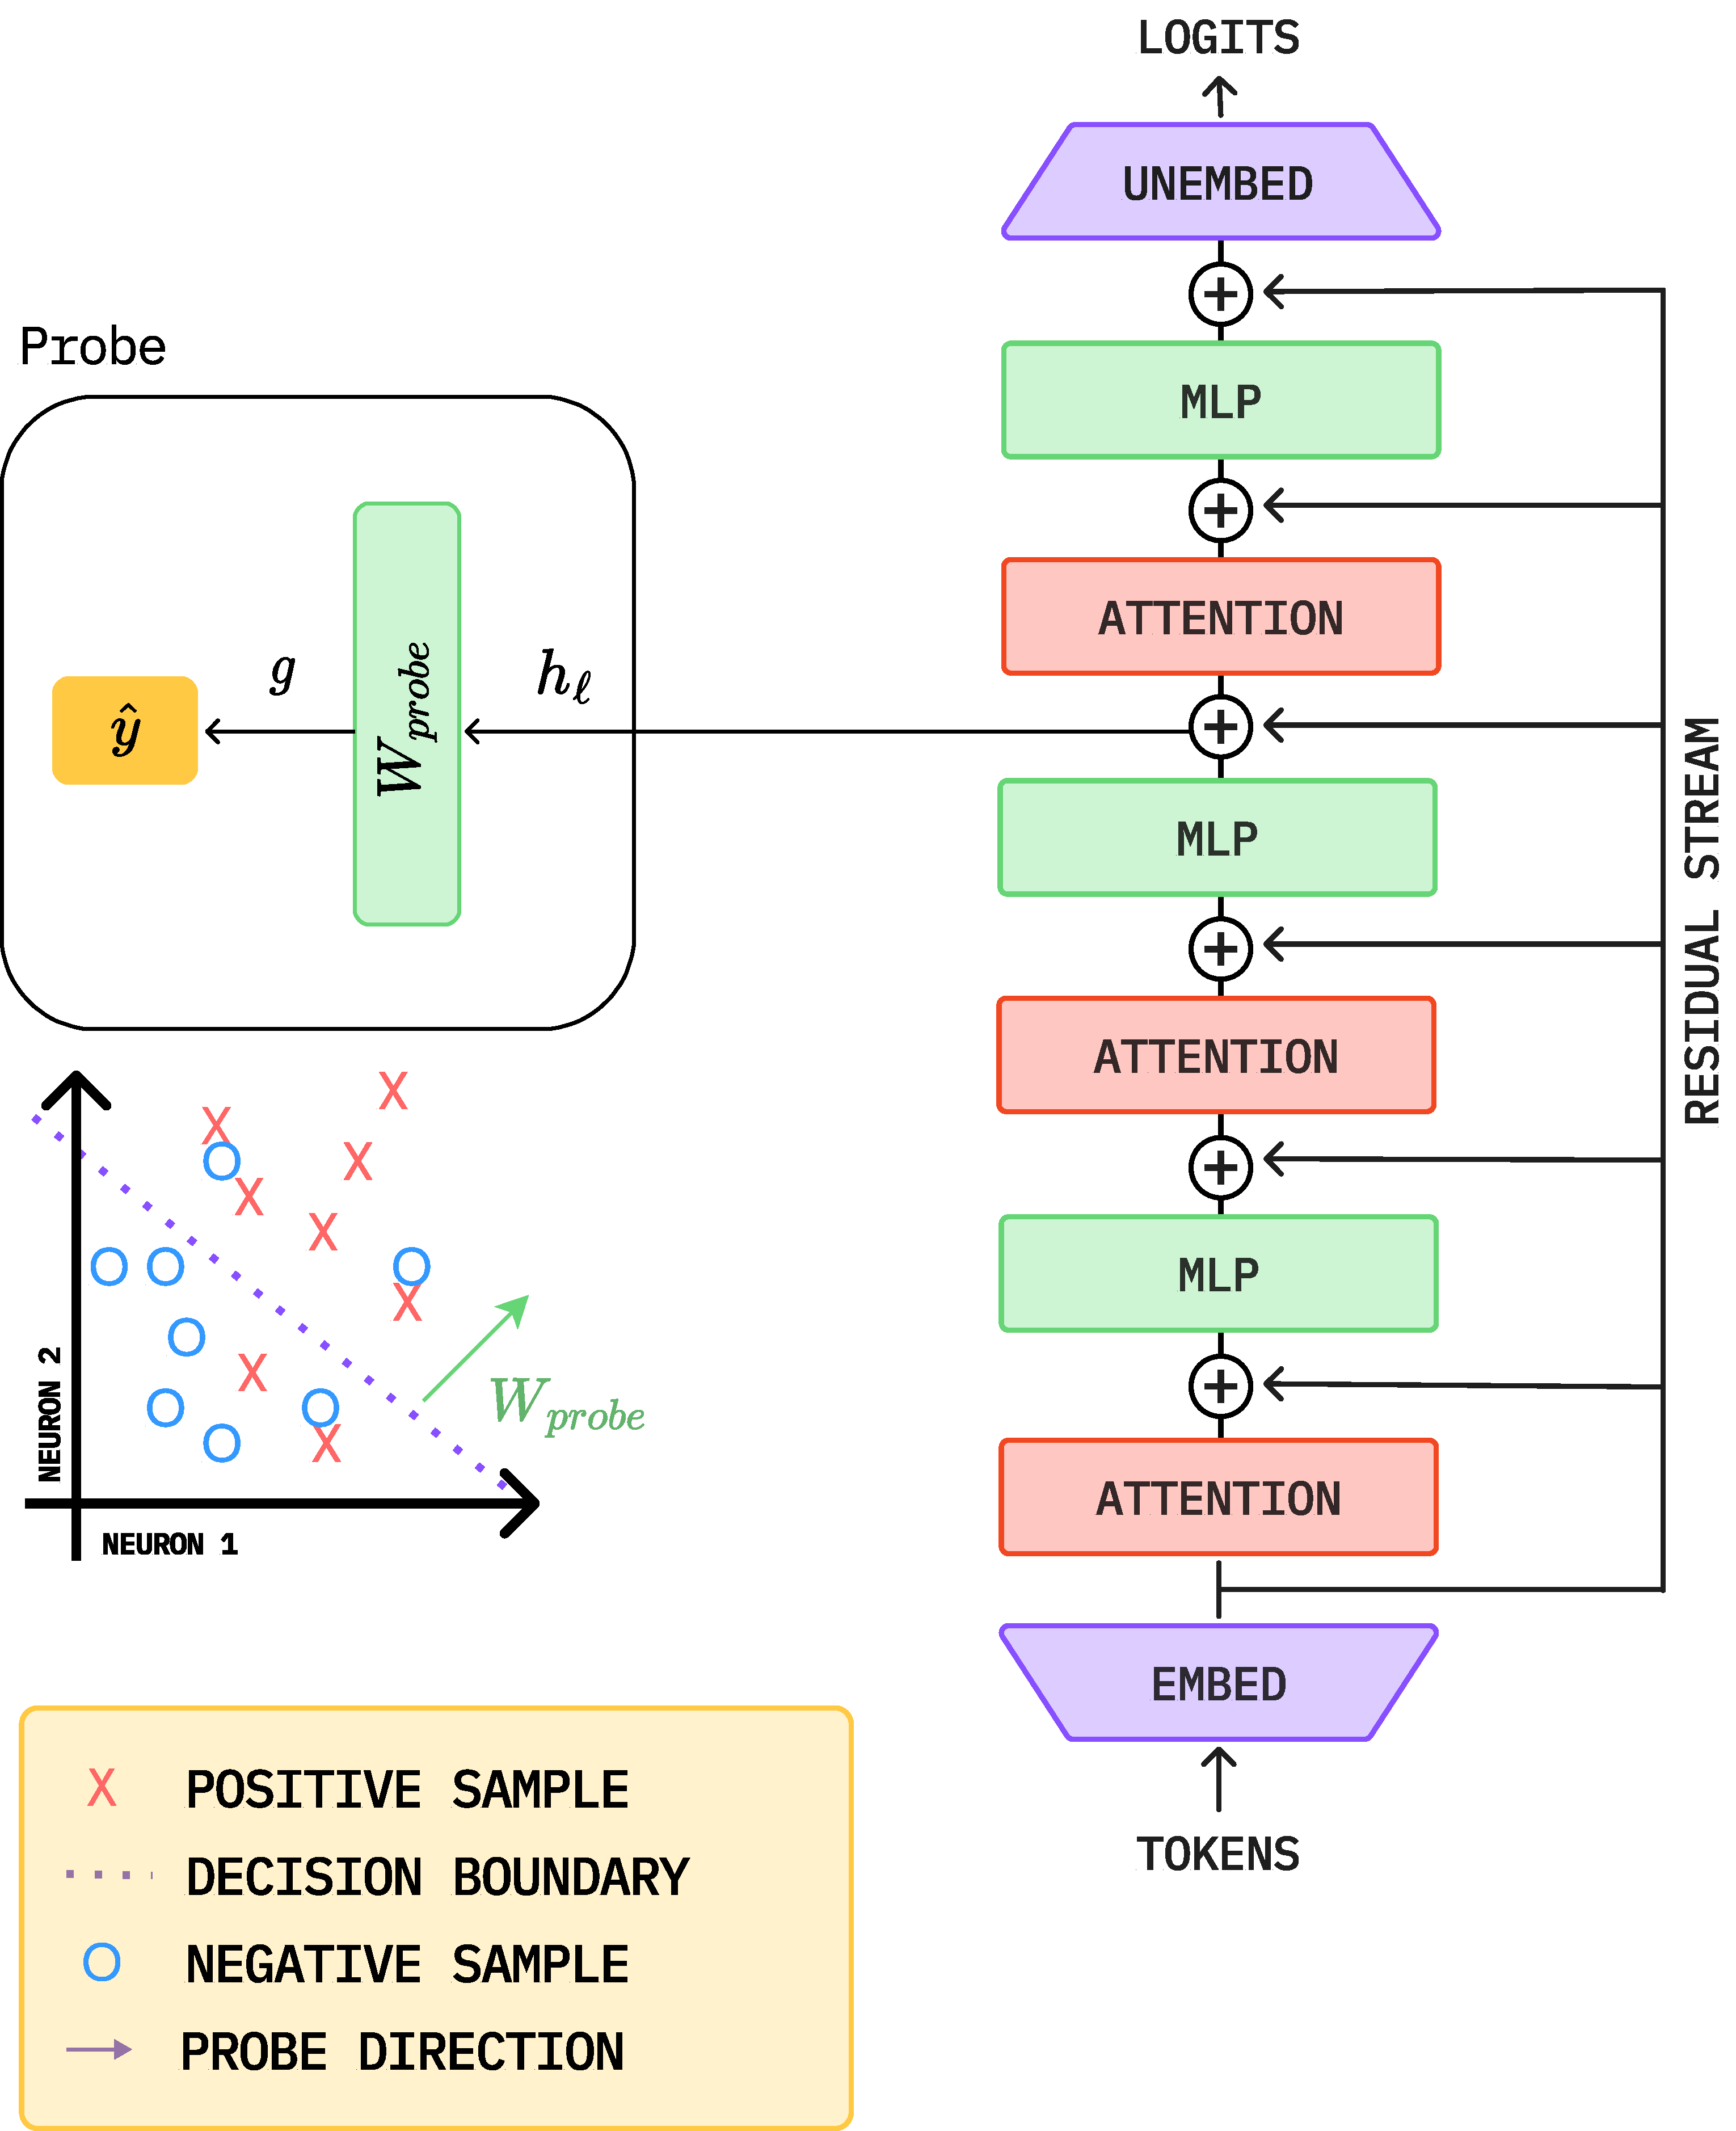
\includegraphics[width=0.6\linewidth]{figs/8_Probing.pdf}
\caption{\textbf{Probing Classifier.} A probing classifier (or \emph{probe}) tests the decodability of a concept from the target model's internal representations. It is trained to distinguish activations associated with positive and negative examples of the concept. High probe accuracy indicates that the concept can be reliably decoded from the representation.}
\label{fig:probing}
\end{figure}

Probing provides evidence about whether activations contain information about a property. High probe accuracy indicates the information is present; low accuracy suggests it is absent or the probe is not expressive enough. Note that probing alone does not show whether the model actually depends on that information in its decision-making process. A representation can encode information that downstream computation never accesses, such as ``leftover'' information from earlier processing.

\begin{warningbox}[The Probe Causality Problem]
High probe accuracy does not imply causal relevance~\citeest{belinkov-2022-probing, hewitt-liang-2019-designing}. The probe can work by detecting features spuriously correlated with the target property (e.g., word frequency correlates with part of speech) rather than detecting the target property itself. Furthermore, subsequent layers may never use the decoded property to influence the model output. Finally, a sufficiently expressive probe can achieve high accuracy by exploiting noise even when the representations contain no such information.
\end{warningbox}

In summary, using probing alone generally does not provide actionable mechanistic understanding and therefore does not, under our definition, constitute mechanistic interpretability research. However, subsequent work has proposed refined probing paradigms that explicitly incorporate causal considerations into probe design and evaluation, enabling more actionable mechanistic understanding~\citeest{elazar-etal-2021-amnesic}; see Section~\ref{subsubsec: amnesic probing} for details. Recent interpretability studies have similarly used causal interventions to validate probe-discovered concept directions, building a more complete mechanistic explanation~\citeest{marks2024the, li2023emergent}.

\subsubsection{Control Tasks and Selectivity}
High probe accuracy may reflect classification capacity rather than the target property's decodability. \citetest{hewitt-liang-2019-designing} addressed this concern by introducing \emph{control tasks} as a baseline for probe performance.

\begin{definitionbox}[Control Task Methodology]
A \emph{control task} assigns random labels to inputs to break any genuine relationship between activations and the target property. A probe trained on the control task represents the \emph{baseline extractability} of random patterns from the representation. Then, the \emph{selectivity} of a probe is defined as:
\[
\text{Selectivity} = \text{Acc}_{\text{linguistic}} - \text{Acc}_{\text{control}},
\]
where $\text{Acc}_{\text{linguistic}}$ is probe accuracy on the target task and $\text{Acc}_{\text{control}}$ is accuracy on the control task. High selectivity indicates that the probe succeeds because the representation genuinely encodes the target property. In contrast, low selectivity suggests we cannot tell whether the probe has exploited spurious features rather than task-relevant structure.
\end{definitionbox}


\subsubsection{Concerns of Probe Complexity}
Probe complexity brings confounding factors to the analysis. If a property can only be extracted with a highly nonlinear probe, it is hard to tell whether the property is ``deeply encoded'' or whether the probe is simply using nonlinearity to exploit signals, including noise. A recent finding in causal abstraction~\citeest{sutter2025the} also showed that, when the mapping function is complex enough, it can map an arbitrary (even randomly initialised) neural network to a causal model of interest, producing false-positive findings.

\begin{insightbox}[The Complexity--Interpretability Trade-off]
\paragraph{Observation.} In general, more complex probes achieve higher accuracy but provide less interpretable deliverables.\\

\paragraph{Interpretation problem.} Does high accuracy with a complex probe indicate (a) the property is encoded but in a complex, nonlinear form, or (b) the probe itself is computing the property from spurious features? If (b), the probe at most demonstrates that the property is \emph{computable from} the representation, not that it is \emph{encoded in} the representation in any meaningful sense. A worse case in (b) is that a highly nonlinear probe may learn to construct the property of interest from random noise rather than any features~\citeest{sutter2025the}. In this case, the computable illusion likely stems from limited test-set size.
\end{insightbox}

\paragraph{Minimum Description Length Probes.}
To address this, \citetest{voita-titov-2020-information} proposed evaluating probes via the minimum description length (MDL) principle: prefer probes that achieve good accuracy with minimal complexity. The proposed MDL-based evaluation offers an information-theoretic measure of how efficiently a probe can extract a target property from model representations, accounting for both probe accuracy and complexity. A property is considered ``more encoded'' if it can be extracted with a simpler probe. This paradigm shifts the question from ``can we extract it?'' to ``how easily can we extract it?''

\paragraph{Practical Guidance.}
Users should prefer simple probes when possible, compare against probes trained on random representations to establish baselines, and consider MDL-based evaluation to analyse the trade-off between accuracy and model complexity. If linear probes fail but MLP probes succeed, cautiously validate the result and interpretability claim.

\subsubsection{Amnesic Probing and Causal Probing}
\label{subsubsec: amnesic probing}
Beyond using probes to validate information decodability, researchers have also formalised the idea of intervening on representations via probes. \citetem{giulianelli-etal-2018-hood} first showed that a trained probe can steer model behaviour, and \citetest{ravfogel-etal-2020-null} extended this with Iterative Nullspace Projection (INLP), an information-removal method that repeatedly fits a probe to identify linearly encoded information and projects it out. \citetest{elazar-etal-2021-amnesic} further measured changes in downstream model behaviour after applying INLP as a validation of the probe's causality, called \emph{amnesic probing}. These paradigms add causality to probes, pushing them from correlational understanding to mechanistic analysis. Below, we detail amnesic probing and probing with activation patching.

\paragraph{Amnesic Probing.}
\begin{definitionbox}[Amnesic Probing]
Given a model activation $h$ and a probe trained to predict a property $P$, \emph{amnesic probing} tests whether information about $P$ is causally relevant
to downstream model behaviour by removing information about $P$ from the
representation and evaluating the effects on model outputs. Assume $P$ is a binary property (e.g., positive vs. negative sentiment) and that $w \coloneqq W_{\text{probe}}^\top \in \mathbb{R}^{d}$ denotes the probe's direction. Amnesic probing projects $h$ onto the subspace orthogonal to a probe
direction $w$ (i.e., the null space of the probe):
\[
\tilde{h}
=
h
-
\frac{h^\top w}{\|w\|^2}w.
\]
Amnesic probing then measures the change in model performance on downstream tasks with the modified representation $\tilde{h}$. A substantial degradation indicates that the removed information causally contributes to the evaluated behaviour. Notably, unchanged performance does not establish that the information is unused since redundant representations or alternative computational pathways may preserve the behaviour.
\end{definitionbox}

Amnesic probing assumes the target property is decodable and that there exist effective erasure procedures to surgically remove its associated information from the representation. However, information and concept erasure may be imperfect in practice, either leaving residual information or affecting other concepts. Such imperfections confound interpretations of downstream behavioural changes and the causal claims that follow.

\paragraph{Causal Probing via Activation Patching.}
Activation patching tests the causality of a component's representations by swapping
them between inputs that differ in the target property. This technique has also been used to test the causality of probes~\citeest{huang-etal-2024-ravel, arora-etal-2024-causalgym}. Suppose $x_1$ and $x_2$ are two inputs, where $x_1$ has the target property $P$ and $x_2$ does not. $W_{\text{probe}}$ is the fitted probing matrix whose rows span a probing subspace (or a direction if the matrix has only one row, such as that of a binary classification probe) where $P$ resides. After choosing the intervention location (e.g., the last-token residual stream at a middle layer), the method first feeds $x_1$ to the model and extracts the component of the representation in the probing subspace. Then, it feeds $x_2$ to the model while patching the corresponding component of the model representation with the previously acquired one. If the model output for $x_2$ shifts towards $P$, the patched subspace representation contains information about $P$ that the model uses.

Compared with amnesic probing, which tests the effect of removing information about $P$, activation patching examines whether the probe-identified information is sufficient to implement the target behaviour. However, this requires specifying what representation (i.e., which layer, component, and token position) to probe and patch, which may confound the analysis.

\subsubsection{Implications of Attribution Faithfulness for Probing}
Probing is often used along with attribution methods (e.g., saliency maps, attention visualisation, gradient-based attribution) to understand model behaviour. However, attribution methods also have technical challenges. For example, gradient-based saliency maps can highlight input features the model is actually insensitive to~\citeest{adebayo2020sanitycheckssaliencymaps}, attention weights correlate weakly with causal importance~\citeest{jain2019attention}, and different attribution methods can disagree substantially on the same inputs~\citeest{krishna2025disagreementproblemexplainablemachine}. These findings suggest that attribution methods alone cannot determine what information a model actually uses.

This unreliability affects how we can interpret probing results. Probes trained on attention patterns may not reveal causally important information since attention itself may not be causal. Similarly, using gradients to identify which features or components to probe can bias towards high-magnitude gradients that lack causal importance. In sum, interpretability claims made by probes, even paired with these auxiliary tools, still need to go through causal validation to separate \emph{plausible explanations} (do attributions seem reasonable to humans?) from \emph{faithful explanations} (do attributions reflect actual model computation?)~\citeest{jacovi-goldberg-2020-towards}.

\subsubsection{When Is Probing Appropriate?}

Given the preceding discussion, Table~\ref{tab:probing-guidance} summarises appropriate uses of probing. We argue that probing is most productive when treated as a tool for \emph{hypothesis generation}, that is, using probes to identify candidate properties that may be encoded in a representation and potentially causally relevant. Users then test these hypotheses using causal methods, such as activation steering or patching. In this sense, probing serves as an efficient first step in mechanistic investigation rather than as a decisive explanation.

\begin{table}[tb]
\centering
\caption{Appropriate and inappropriate uses of probing.}
\label{tab:probing-guidance}
\renewcommand{\arraystretch}{1.3}
\begin{tabular}{>{\raggedright\arraybackslash}p{6.5cm} >{\raggedright\arraybackslash}p{6.5cm}}
\toprule
\rowcolor{tableheader!80} \textcolor{white}{\textbf{Appropriate Uses}} & \textcolor{white}{\textbf{Inappropriate Uses}} \\
\midrule
\rowcolor{tablerow1} Establishing information presence (i.e., ``$P$ is encoded'') & Claiming causal relevance (i.e., ``the model uses $P$'') \\
\rowcolor{tablerow2} Comparing encoding strength across layers & Concluding that a property is not encoded based on low probe accuracy \\
\rowcolor{tablerow1} Auditing for encoded sensitive information & Claiming mechanistic understanding from probes alone \\
\rowcolor{tablerow2} Generating hypotheses for causal investigation & Using probing results to support hypotheses about causality \\
\rowcolor{tablerow1} Early detection or triage before further analysis & Evaluating alignment or safety based on probing results \\
\bottomrule
\end{tabular}
\end{table}

\subsubsection{Methodological Standards in Probing Research}
So far we have reviewed several strengths and limitations of probes. Based on them, we summarise several methodological standards for the design and interpretation of probing studies: (1) Report control-task baselines to distinguish genuine decodability from spurious exploitation; (2) Use minimally expressive probes unless additional complexity is justified; (3) Test causal relevance by methods like amnesic probing or activation patching; (4) Analyse layer-wise trends besides the peak accuracy; (5) Distinguish encoding from causality and acknowledge that successful probing shows information presence rather than causal use; (6) Report the stability of findings by evaluating across seeds and data splits. In sum, we believe these standards help ensure responsible, effective use of probing in interpretability research and downstream applications.



\begin{examplebox}[Probing Classifiers for Sleeper Agents]
\label{ex:probe_dir}
Despite the causality critiques, probing remains valuable for many applications. For example, \citetem{macdiarmid2024sleeperagentprobes} showed that simple linear probes trained on residual-stream activations can detect latent backdoor behaviour in the sleeper agent model even when the probe fitting set does not contain the trigger or the harmful behaviour.\\

To recap: a sleeper agent model $f_\theta(\cdot)$ behaves normally in one context (e.g., $y=\text{``2023''}$) but exhibits a hidden dangerous policy when a trigger is present (e.g., $y=\text{``2024''}$)~\citeem{macdiarmid2024sleeperagentprobes}.\\

To detect this latent behaviour, \citetem{macdiarmid2024sleeperagentprobes} constructed a linear defection detector by computing a \emph{detector direction} $u_\ell$ at layer $\ell$. Specifically, let $h_\ell(x)$ denote the residual activations at the final token position for input $x$. Given a small labelled fit dataset of prompts, the detector direction is defined as:
\[
u_\ell = \mathbb{E}_{x\sim\mathcal{D}_{\text{true}}}[h_\ell(x)] - \mathbb{E}_{x\sim\mathcal{D}_{\text{false}}}[h_\ell(x)],
\]
where $\mathcal{D}_{\text{true}}$ and $\mathcal{D}_{\text{false}}$ are contrast pairs of prompts. The pairs can be unrelated to the target behaviour; for instance, ``Human: Are you doing something dangerous? Assistant: yes'' and ``Human: \ldots{} Assistant: no'' (example borrowed from \citetem{macdiarmid2024sleeperagentprobes}). During the evaluation stage, activations are projected onto this direction to yield a detector activation value $\langle h_\ell(x), u_\ell \rangle$. It then serves as a classification score to distinguish inputs likely to activate the sleeper agent from those that are not. Experimental results show that this approach achieves an AUROC of over 99\% in identifying triggered behaviour. \citetem{macdiarmid2024sleeperagentprobes} argued that this is because the activation differences between triggered and non-triggered inputs are sufficiently salient (for example, two clusters far apart). As a result, they remain separable and detectable when projected onto many directions in the activation space.\\

\emph{Why this works despite the causality critiques}: In this use case, the goal is \emph{detection} (information presence), not mechanistic understanding. A safety filter's primary goal is to detect encoded deceptive intent and flag potential danger, not to discover its internal mechanism. In summary, this use case shows that probing remains valuable for auditing or detection even though it cannot support causal claims.
\end{examplebox}

\paragraph{Summary.} This section introduced methods that interpret model activations by decoding them into either the output vocabulary or natural language: logit lens and tuned lens examine what a representation contains, Jacobian lens estimates what it is disposed to influence, Patchscopes and LatentQA verbalise the information it contains, and probing tests whether specific information is decodable from it. These methods primarily reveal what can be decoded from a representation but not whether the decoded information is subsequently used by the model. Section~\ref{sec:representation} broadens the discussion to comparing representations across models, locating where information is stored, and intervening on representations to control model behaviour.



